\subsection{Softening the constraints}
In the QUBO formalism, there are no hard constraints; thus the use of penalty functions in the previous section.
For sufficiently large penalty weights, the optimum will satisfy the desired constraints.
However, precision is a limited resource in quantum annealing~\cite{TODO:D-Wave-precision}; therefore, we would like to determine the smallest sufficient penalty weights.

\begin{figure}[h]
\centering
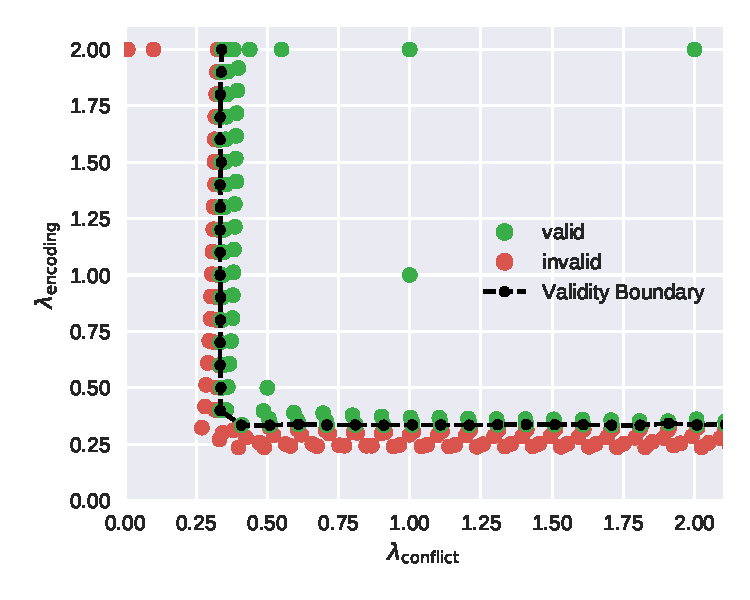
\includegraphics[width=0.45\textwidth]{./pics/validity_boundary_example.pdf}
\caption[Penalty weight phase diagram]{Validity of exact solution to a QUBO extracted from a problem instance with $N_f=7$ flights and $N_c=9$ conflicts in dependence on the choice of the penalty weights, $\lambda_\text{unique}$ and $\lambda_\text{conflict}$. Here, $\Delta_t=6$ and $d_\text{max}=18$.}
\label{fig:penalty_weights}
\end{figure}

For a given instance, we say that a pair of penalty weights $(\weight{conflict}, \weight{encoding})$ is valid if the minimum of the total cost function satisfies both the conflict and encoding constraints when using those weights.
Figure~\ref{fig:penalty_weights} shows the phase space of these penalty weights for a single instance with $7$ flights and $9$ conflicts.
The box-like boundary between valid and invalid penalty weights suggests that the validity of the two penalty weights is independent; 
this box-like boundary is found for all of our instances with up to $7$ flights and $9$ conflicts.
%In order to find these optimal penalty weights, we employed an exact solver
%\footnote{Reference to mapping from QUBO to max sat and to akmaxsat solver} to explore the validity of a solution in dependence on the penalty weights.

One can give an upper bound for the sufficiently large penalty weights by the following considerations.
A minimal violation of the hard constraints yield an additional contribution to the QUBO cost function of $\lambda_\text{unique}$ or $\lambda_\text{conflict}$, respectively.
Such a violation would correspond to single bit flip in the binary delay variables $d_{i\alpha}$.
Therefore the contribution from~\eqref{eqn:departure_delay_model_qubo_departure} would be reduced maximally by 
\begin{equation*}
    \min_\alpha \frac{-\alpha}{d_\text{max}} = - 1    
\end{equation*}
Hence, sufficiently large penalty weights must fulfill the following conditions
\begin{align*}
    \lambda_\text{unique} & > 1 \\
    \lambda_\text{conflict} &> 1 \, .
\end{align*}
This corresponds to a box like shape as it appears in figure~\ref{fig:penalty_weights}.
